\documentclass[entwurf.tex]{subfiles}

\begin{document}
\chapter{Klassendiagramme}
	\section{Bus}
		In dem folgenden Diagramm sieht man den Aufbau des Busses, mit dem Interface für die Publisher und Subscriber sowie den verschiedenen Typen von Messages.
		\begin{figure}[H]
  			\begin{center}
 				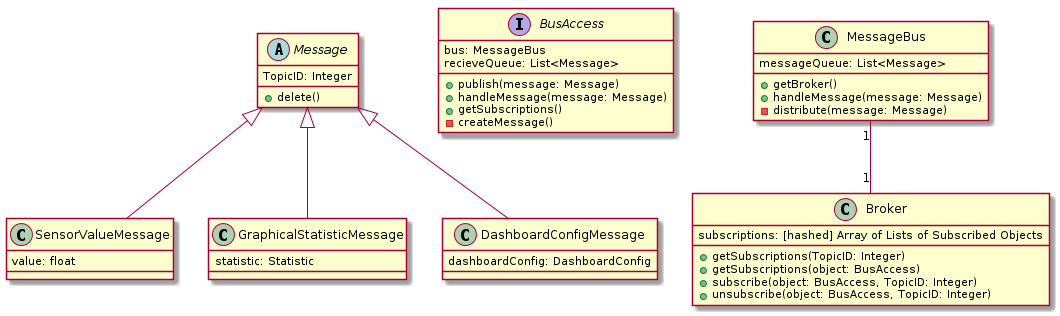
\includegraphics[width=\textwidth]{diagrams/Bus.png}
  				\caption{Bus Klassendiagramm}
  			\end{center}
  		\end{figure}
  		
  	
  	\newpage
  	\section{Virtual Sensors}
		Hier sieht man den Aufbau der Virtuellen Sensoren.
		\begin{figure}[H]
  			\begin{center}
 				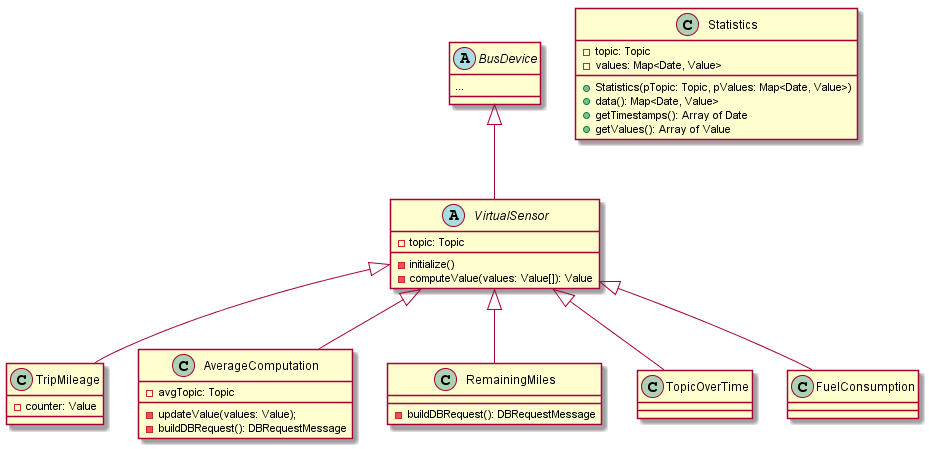
\includegraphics[width=\textwidth]{diagrams/VirtualSensors.png}
  				\caption{Virtuelle Sensoren Klassendiagramm}
  			\end{center}
  		\end{figure}
  	
  	
  	
  	\newpage
  	\section{User Interface}
		In dem folgenden Diagramm sieht man den Aufbau der UI auf der Seite des Terminals
		\begin{figure}[H]
  			\begin{center}
 				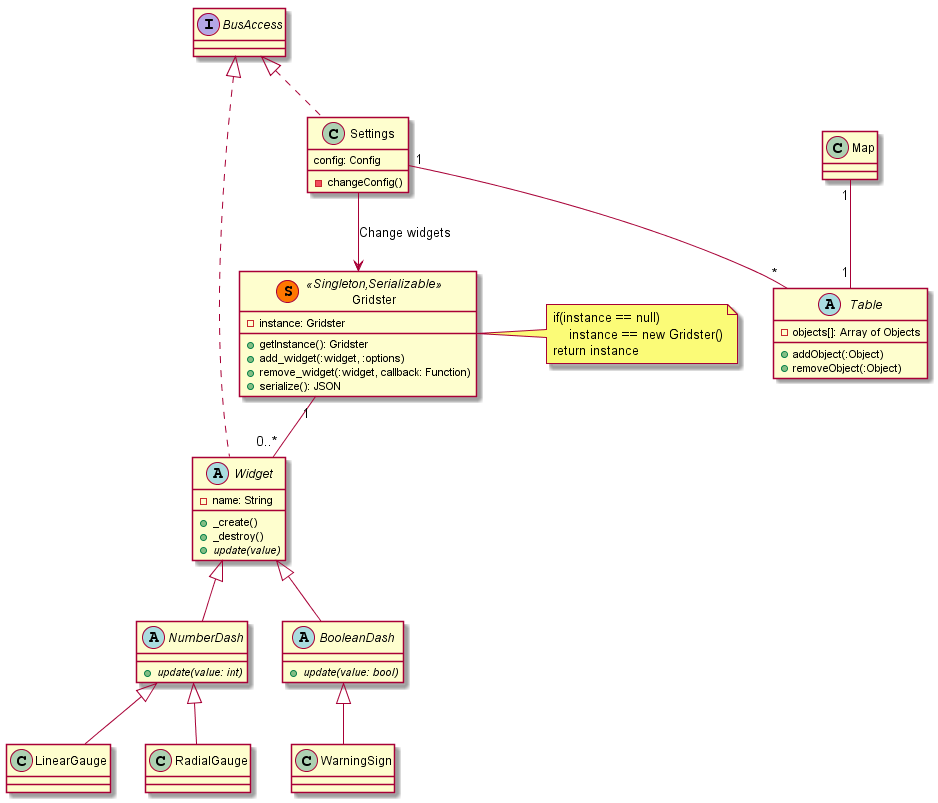
\includegraphics[width=\textwidth]{diagrams/UI.png}
  				\caption{UI Klassendiagramm}
  			\end{center}
  		\end{figure}
  		
  		
  		
  	\newpage
  	\section{Parking Sensor}
		Hier ist zu sehen wie das Rückfahrassistenzsystem aufgebaut ist. Siehe auch %TODO Link sequenzdiagramm
		\begin{figure}[H]
  			\begin{center}
 				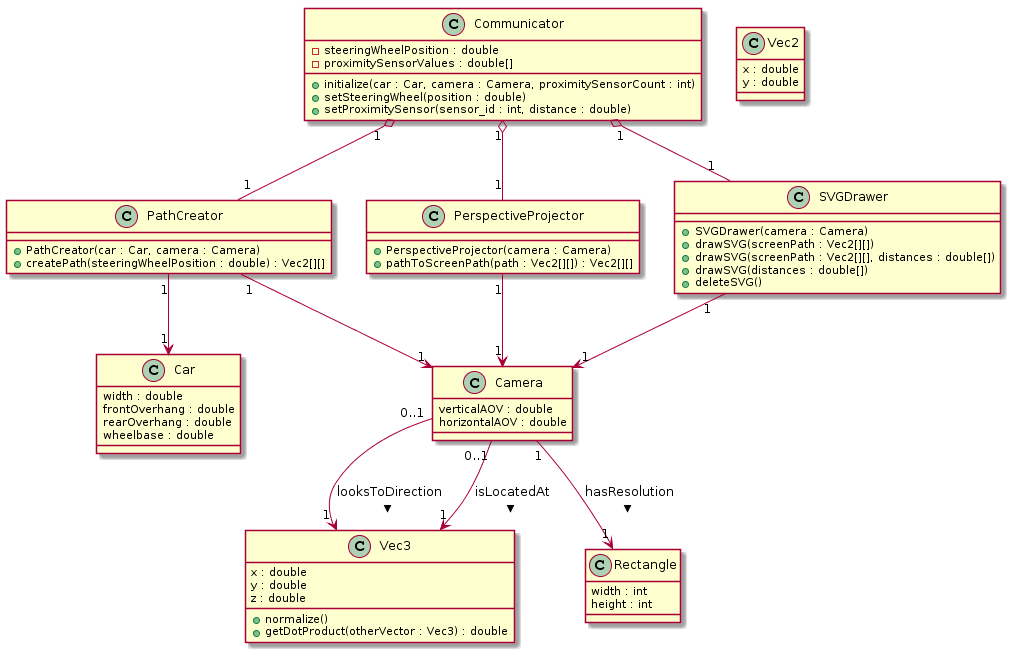
\includegraphics[width=\textwidth]{diagrams/ParkingSensor/class_diagram.png}
  				\caption{Rückfahrsystem Klassendiagramm}
  			\end{center}
  		\end{figure}
  	
  	
\end{document}
